% This file was created by tikzplotlib v0.9.8.
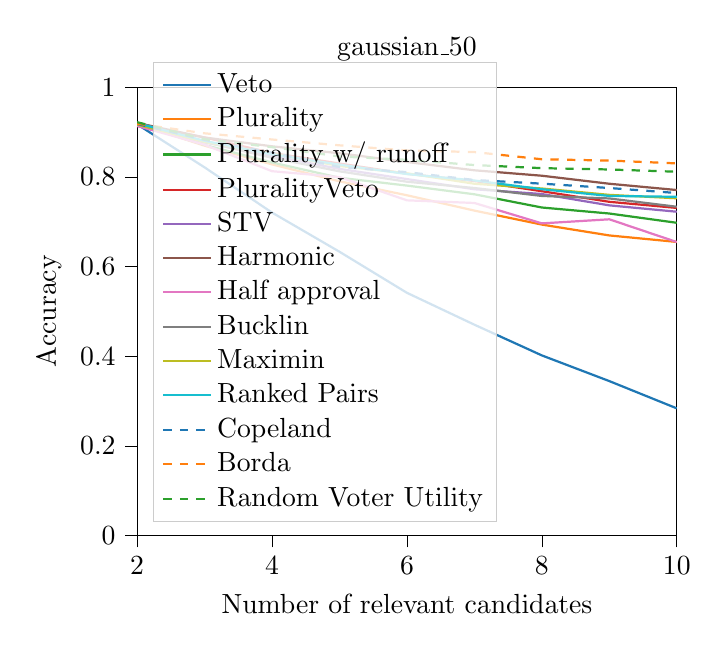
\begin{tikzpicture}

\definecolor{color0}{rgb}{0.12156862745098,0.466666666666667,0.705882352941177}
\definecolor{color1}{rgb}{1,0.498039215686275,0.0549019607843137}
\definecolor{color2}{rgb}{0.172549019607843,0.627450980392157,0.172549019607843}
\definecolor{color3}{rgb}{0.83921568627451,0.152941176470588,0.156862745098039}
\definecolor{color4}{rgb}{0.580392156862745,0.403921568627451,0.741176470588235}
\definecolor{color5}{rgb}{0.549019607843137,0.337254901960784,0.294117647058824}
\definecolor{color6}{rgb}{0.890196078431372,0.466666666666667,0.76078431372549}
\definecolor{color7}{rgb}{0.737254901960784,0.741176470588235,0.133333333333333}
\definecolor{color8}{rgb}{0.0901960784313725,0.745098039215686,0.811764705882353}

\begin{axis}[
legend cell align={left},
legend style={
  fill opacity=0.8,
  draw opacity=1,
  text opacity=1,
  at={(0.03,0.03)},
  anchor=south west,
  draw=white!80!black
},
tick align=outside,
tick pos=left,
title={gaussian\_50},
x grid style={white!69.0196078431373!black},
xlabel={Number of relevant candidates},
xmin=2, xmax=10,
xtick style={color=black},
y grid style={white!69.0196078431373!black},
ylabel={Accuracy},
ymin=0, ymax=1,
ytick style={color=black}
]
\addplot [thick, color0]
table {%
2 0.9171
3 0.821
4 0.7202
5 0.6328
6 0.5412
7 0.4701
8 0.4016
9 0.3443
10 0.2835
};
\addlegendentry{Veto}
\addplot [thick, color1]
table {%
2 0.9181
3 0.8694
4 0.8277
5 0.7899
6 0.7588
7 0.7246
8 0.6934
9 0.6692
10 0.6547
};
\addlegendentry{Plurality}
\addplot [thick, color2]
table {%
2 0.9176
3 0.8711
4 0.832
5 0.7979
6 0.7804
7 0.761
8 0.7315
9 0.7181
10 0.6974
};
\addlegendentry{Plurality w/ runoff}
\addplot [thick, color3]
table {%
2 0.9173
3 0.8876
4 0.8532
5 0.8296
6 0.8066
7 0.7906
8 0.7678
9 0.7442
10 0.7306
};
\addlegendentry{PluralityVeto}
\addplot [thick, color4]
table {%
2 0.9133
3 0.8766
4 0.8468
5 0.8176
6 0.7949
7 0.7722
8 0.7616
9 0.7363
10 0.7221
};
\addlegendentry{STV}
\addplot [thick, color5]
table {%
2 0.9201
3 0.8877
4 0.868
5 0.8525
6 0.833
7 0.8145
8 0.8024
9 0.7845
10 0.7705
};
\addlegendentry{Harmonic}
\addplot [thick, color6]
table {%
2 0.9136
3 0.8715
4 0.8125
5 0.7994
6 0.7475
7 0.7416
8 0.6961
9 0.7052
10 0.6545
};
\addlegendentry{Half approval}
\addplot [thick, white!49.8039215686275!black]
table {%
2 0.921
3 0.878
4 0.8424
5 0.8122
6 0.789
7 0.775
8 0.7573
9 0.7517
10 0.7332
};
\addlegendentry{Bucklin}
\addplot [thick, color7]
table {%
2 0.9165
3 0.8778
4 0.852
5 0.824
6 0.8078
7 0.7845
8 0.7739
9 0.7597
10 0.7521
};
\addlegendentry{Maximin}
\addplot [thick, color8]
table {%
2 0.9195
3 0.8803
4 0.8502
5 0.8271
6 0.8061
7 0.7918
8 0.7723
9 0.7573
10 0.7554
};
\addlegendentry{Ranked Pairs}
\addplot [thick, color0, dashed]
table {%
2 0.9179
3 0.8824
4 0.8539
5 0.8217
6 0.8104
7 0.7929
8 0.7847
9 0.775
10 0.7638
};
\addlegendentry{Copeland}
\addplot [thick, color1, dashed]
table {%
2 0.9185
3 0.897
4 0.8832
5 0.8702
6 0.8587
7 0.8552
8 0.8391
9 0.8362
10 0.8299
};
\addlegendentry{Borda}
\addplot [thick, color2, dashed]
table {%
2 0.9218
3 0.8838
4 0.8661
5 0.8454
6 0.8379
7 0.8262
8 0.8193
9 0.8163
10 0.8113
};
\addlegendentry{Random Voter Utility}
\end{axis}

\end{tikzpicture}
